\chapter{Peruskäsitteitä}

\section{Tyyppijärjestelmien luokitteleminen}
Ohjelmointikielten tyyppijärjestelmien jakaminen staattisesti ja dynaamisesti
tyyppitarkastettuihin perustuu ohjelman kehitysvaiheeseen jossa tarkastaminen
tapahtuu. Staattisella tyyppitarkastamisella viitataan ohjelman tyyppien
analyysiin ennen sen suorittamista, esimerkiksi käännösaikana, kun taas
dynaaminen tyyppitarkastus varmistaa arvojen tyyppien oikeellisuuden ohjelmaa
suoritettaessa. Tyyppijärjestelmät voidaan jaotella myös muiden
ominaisuuksien perusteella, esimerkiksi vahvoihin ja heikkoihin
tyyppijärjestelmiin. Näiden termien merkitys ei ole tarkasti määritelty,
mutta yleisesti niillä viitataan tapaan jolla kieli käsittelee tarkoitetusta
poikkeavat, virheelliset tyypit \cite{CornellTransitionToOO}. Vahvasti
tyypitetyssä kielessä tällainen aiheuttaisi käännös- tai ajonaikaisen
virheen, kun taas heikosti tyypitetyssä kielessä arvoille voitaisiin tehdä
implisiittisiä tyyppimuunnoksia niiden yhteensopivuuden saavuttamiseksi.

JavaScript on dynaamisesti tarkastettu, heikosti tyypitetty kieli.
Esimerkiksi ohjelma \inlinecode{\dblquoted{teksti}.potenssiin(3)} antaa
staattisesti tyyppitarkastetussa kielessä virheen jo käännösaikana, mikäli
metodia \inlinecode{potenssiin} ei ole tekstityyppisille arvoille määritetty.
JavaScriptiä suorittava ympäristö sen sijaan hyväksyisi ohjelman ja sallisi
sen suorittamisen. Virhe olemattoman metodin kutsumisesta ilmenisi vasta jos
ohjelman suoritus evaluoi kyseisen ilmaisun. Lisäksi esimerkiksi ilmaisu
\inlinecode{\dblquoted{teksti} + 2} ei aiheuttaisi virhettä edes 
suoritusaikana, sillä heikoille tyyppijärjestelmille ominaisesti JavaScript
muuttaisi numeron 2 string-muotoon ennen summausoperaation arviointia. Tässä
tutkielmassa keskitytään lähinnä JavaScriptin tyyppien staattiseen ja
dynaamiseen, eli käytännössä käännös- ja ajonaikaiseen tarkastamiseen. Jotkin
esitellyistä työkaluista myös tiukentavat kielen sallimia operaatioita siten,
että esimerkiksi yllä esitettyä \inlinecode{\dblquoted{teksti} + 2} ohjelmaa
ei enää sallittaisi. Monia muita heikoille tyyppijärjestelmille
tavallisia ominaisuuksia jää kuitenkin tarkistamatta.

\begin{figure}
\centering
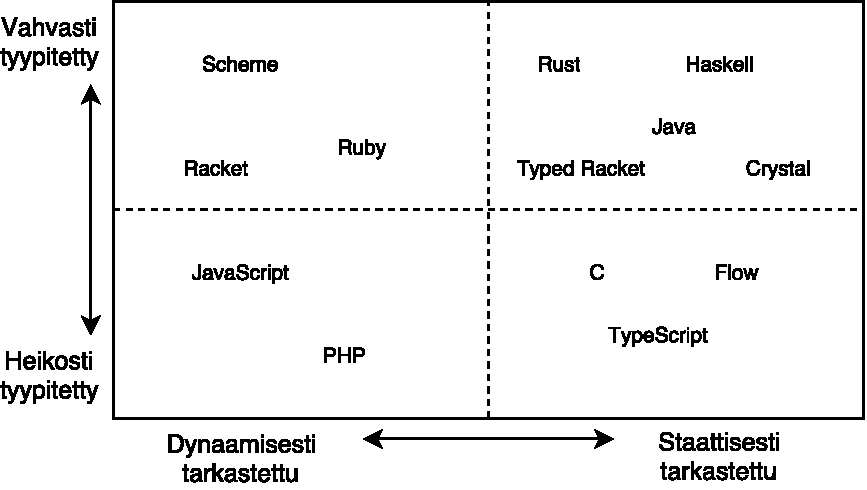
\includegraphics{images/type-systems.pdf}
\caption{Tyyppijärjestelmät eri ohjelmointikielissä}
\end{figure}

\section{ECMA-262, EcmaScript ja JavaScript}
``EcmaScript'' on ECMA-262 standardin määrittelemä ohjelmointikieli
\cite{JavaScriptLanguageResources, Ecma262}, jonka kehityksestä vastaa
organisaatio Ecma International. ``JavaScript'' on Oraclen omistama
tavaramerkki jolla viitataan EcmaScript-kielen osittaisiin tai täydellisiin
toteutuksiin\cite{JavaScriptLanguageResources}. Historiallisista syistä termejä
``JavaScript'' ja ``EcmaScript'' käytetään usein keskenään vaihtokelpoisesti.
Tässä tutkielmassa termillä ``JavaScript'' viitataan ECMA-262:den kahdeksannen
version mukaiseen EcmaScriptiin, jota kutsutaan myös nimellä EcmaScript 2017.

\section{TypeScript}
TypeScript on Microsoftin luoma ohjelmointikieli, jonka tarkoitus on
auttaa JavaScript-ohjelmien kehitystä staattisen tyyppijärjestelmän avulla.
Se on EcmaScriptin ylijoukko (superset) \cite{TypeScriptSpec} ja jatkaa
JavaScriptin syntaksia tyyppimäärittelyihin käytettävällä
annotaatiosyntaksilla. Jokainen validi JavaScript-ohjelma on syntaksiltaan ja
ajonaikaiselta käyttäytymiseltään validi TypeScript-ohjelma. TypeScript
kuitenkin lisää kehitykseen käännösvaiheen, jossa ohjelman tyyppien
oikeellisuus tarkastetaan staattisesti. TypeScript koodi käännetään
JavaScriptiksi, joka puolestaan voidaan suorittaa selaimissa tai muissa
JavaScriptin suoritusympäristöissä. TypeScript kääntäjän voi myös määrittää
muokkaamaan tulostettava koodi yhteensopivaksi vanhempien
EcmaScript-standardien kanssa, mikä on hyödyllistä jos ohjelman on tarkoitus
tukea sellaisia suoritusympäristöjä jotka eivät tue uusinta EcmaScriptin
versiota.

\section{Flow}
Flow on Facebookin kehittämä työkalu, joka TypeScriptin tavoin jatkaa
JavaScriptin syntaksia staattisesti tarkastettavilla tyyppimäärittelyillä.
Flow itsessään ei sisällä kääntäjää, vaan keskittyy yksinomaan ohjelman
tyyppiturvallisuuden tarkastamiseen. Koodiin lisätyt tyyppimääritykset on
kuitenkin poistettava ennen kuin JavaScript-ohjelma voidaan suorittaa. Tähän
tarkoitukseen voidaan käyttää esimerkiksi Babel-kääntäjää, joka poistaa
Flow-tyyppimäärittelyt ja muokkaa JavaScript-koodin yhteensopivaksi toivotun
EcmaScript-version kanssa \cite{FlowInstallation}.

\section{Closure kääntäjä}
Googlen Closure kääntäjä on käännöstyökalu, jonka pääasiallinen tarkoitus
on minimoida ja optimoida JavaScript-koodia käännösvaiheessa ennen tuotantoon
siirtämistä. Closure sisältää kuitenkin myös tuen tyyppivirheiden
tarkastamiselle käännösvaiheessa \cite{ClosureCompiler}. Tyypit annotoidaan
erityisellä JSDoc-pohjaisilla dokumentaatiokommenteilla. Koska annotaatiot
ovat kommenteissa eivätkä erityisenä syntaksina muun suoritettavan koodin
joukossa, Closure-annotoitua JavaScriptiä ei tarvitse kääntää ennen sen
suorittamista \cite{annotatingJSforClosure}.